\chapter{Precision estimation tests}
The automated assembly system has a number of properties in terms of precision:
\begin{enumerate}
\item Motion stage movement repeatability.
\item Image acquiring repeatability.
\item Precision of pattern recognition.
\item Possible movements of the sensors while picking them up and down with the vacuum pick up tool.
\item \ldots
\end{enumerate}

\section{Pattern recognition precision tests}

To investigate the pattern recognition precision the folowing tests were done.  \ldots
\subsection{Pattern recognition on the painted corner of a glass dummy}
Thin pieces of glass with a silver painted corner (Figure \ref{fig:painted_corner}) were used for the tests as an approximation of a silicon sensor. This decision was made due to the fact that real sensors costs a lot and during tests there is a high chance to break them. Fortunately, even none of the glass samples were breaken.

\begin{figure}[ht]\centering
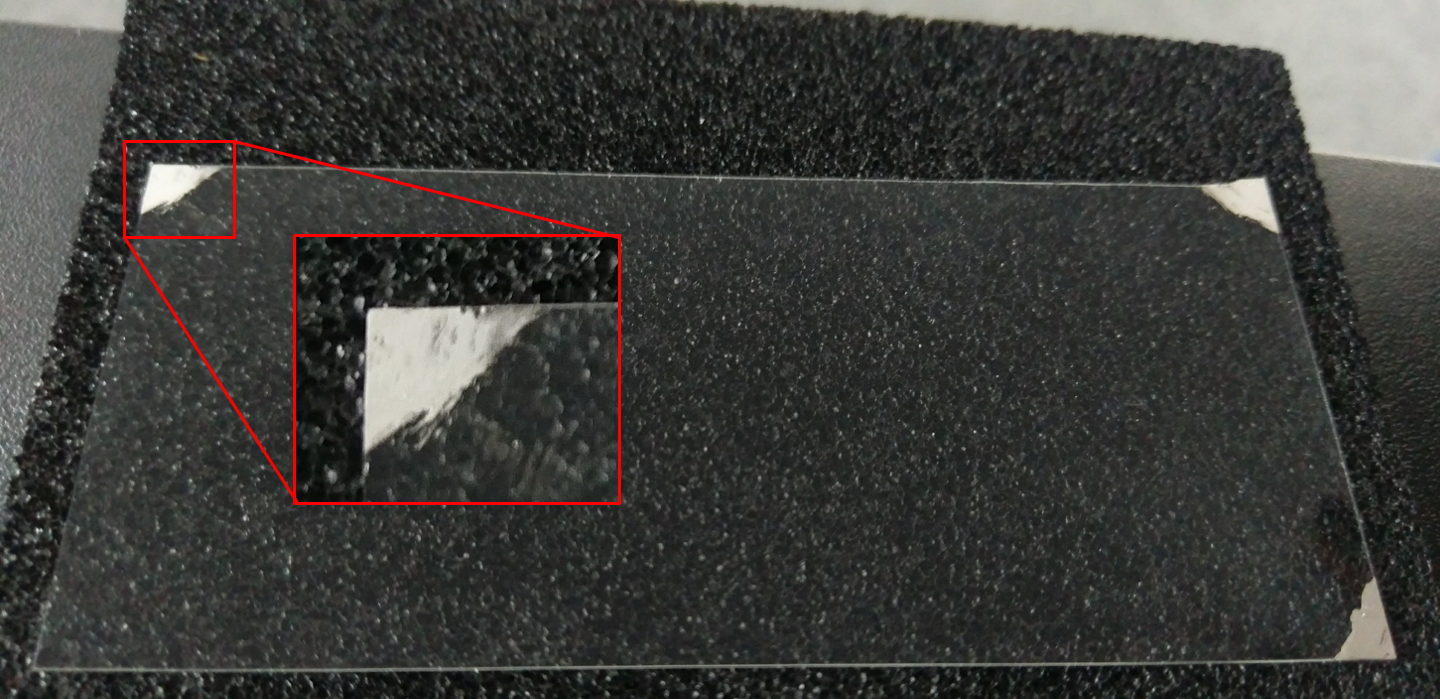
\includegraphics[width=0.8\linewidth]{Data/Precision_tests/Painted_corner.png}
\caption{Glass sample with silver painted corner.}
\label{fig:painted_corner}
\end{figure}

The step-by-step outline of this test is listed below:
\begin{enumerate}
\item Move to the image acquiring position.
\item Acquire Image and run pattern recognition.
\item Move aside for 5mm \underline{in all axes (?)}.
\item Move to the image acquiring position.
\item Acquire Image and run pattern recognition.
\item Save data of the current iteration and go to the next one.
\end{enumerate}

...Results...

\subsection{Pattern recognition on the marker of the dummy sensor}

The same test, but with dummy silicon sensor and real marker on it, was done. Before the test marker was aligned as much close to zero degrees as possible. At the Figure \ref{fig:thresholded_marker} one can see that the edge of the marker after applying Threshold is almost perfect (+/- one pixel). This fact itself is already a proof that Threashold step of pattern recognition is feasible.

\begin{figure}[ht]\centering
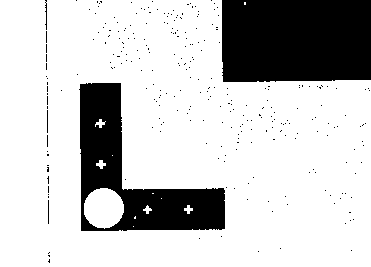
\includegraphics[width=0.8\linewidth]{Data/Precision_tests/Thresholded_marker.png}
\caption{Sensor marker after applying Threshold.}
\label{fig:thresholded_marker}
\end{figure}

The destribution of X and Y coordinates are shown on the Figure XX
The results of the test is shown on the Figure ...





A screenshot of the application during the test is shown on the Figure \ref{fig:marker_pattern_recognition_screenshot}. On the pattern recognition curve one can see that exactly at 0 degree there is a underline{fluctuation (a short upward shot) (?)}. 

\begin{figure}[ht]\centering
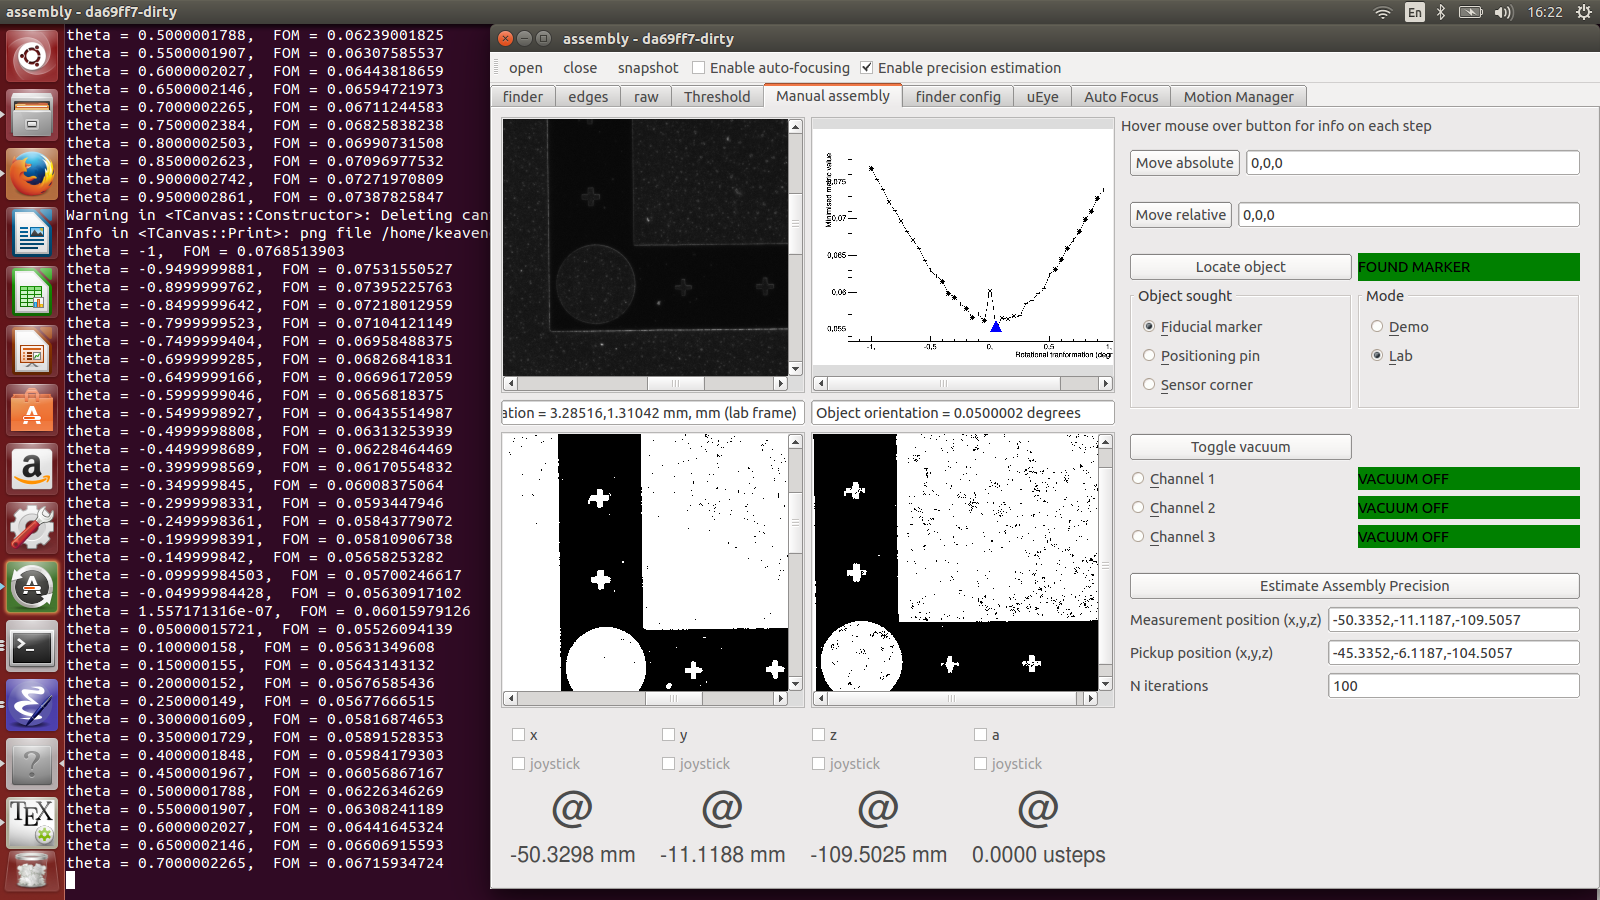
\includegraphics[width=0.8\linewidth]{Data/Precision_tests/Marker_pattern_recognition_screenshot.png}
\caption{Screenshot of application during precision extimation test with dummy silicon sensor and marker on it.}
\label{fig:marker_pattern_recognition_screenshot}
\end{figure}

\section{Arm and camera movements repeatability }

1) Make a photo
2) Move aside
3) Move back
4) Make control photo

\section{Vaccuum pick-up and -down precision}

0) Move to measurement position
1) Corner position
2) Move to pre-pickup position (!)
3) Move to pickup
4) Toggle vacuum 
5) Move up
6) Move down
7) Release vacuum
8) Move to pre-pick-up
9) Move to measurement position
10) Corner position

